\documentclass[aspectratio=169,t,11pt,table]{beamer}
\usepackage{../includes/slides,../includes/math}
\definecolor{accent}{HTML}{2B5269}
\definecolor{accent2}{HTML}{9D2235}

\title{Regression Methods}
\subtitle{\it  ECON 5753 — University of Arkansas}
\date{Sprint 2025}
\author{Prof. Kyle Butts}

\NewDocumentCommand{\logistic}{o g}{%
  \textrm{logistic}\IfValueT{#1}{_{#1}}{\left(#2\right)}
}

\begin{document}

% ------------------------------------------------------------------------------
\begin{frame}[noframenumbering,plain]
\maketitle
\end{frame}
% ------------------------------------------------------------------------------

\begin{frame}{Theoretical Results from Last Time}
  \begin{enumerate}
    \item Derive the OLS estimator $\hat{\beta}_{\text{OLS}} = (\bm{W}' \bm{W})^{-1} \bm{W}' y$
    
    \bigskip
    \item Derive the sample distribution of $\hat{\beta}_{\text{OLS}}$
    $$
      \hat{\beta}_{\text{OLS}} \sim \mathcal{N}(\beta_0, \ (\bm{W}' \bm{W})^{-1} \bm{W}' \Sigma \bm{W} (\bm{W}' \bm{W})^{-1})
    $$
    
    \bigskip
    \item Forecasting $w' \hat{\beta}_{\text{OLS}}$ and $w' \hat{\beta}_{\text{OLS}} \sim \mathcal{N}(w' \beta_0, \ w' V_{\hat{\beta}_{\text{OLS}}} w)$
    
    \bigskip
    \item Marginal (predictive) effects, $\frac{\partial}{\partial x_\ell} \hat{f}(X) = \sum_{k=1}^K \frac{\partial}{\partial x_\ell} g_{k}(X) \hat{\beta}_{\text{OLS}, k}$
  \end{enumerate}
\end{frame}

\begin{frame}{This time}
  The rest of this topic will cover various practical uses of regression:
  \begin{itemize}
    \item Interpreting regression coefficients

    \item Different explanatory variables to include in $W_i$ and how to interpret them
    
    \begin{itemize}
      \item Polynomials, Indicators, Discrete Variables, Bins, Splines
    \end{itemize}

    \item Interactions

    \item Partially linear model
    
    \item $\log$ transformed variables
  \end{itemize}

  
  \bigskip
  Basically, this set of slides is the \emph{applied} half of cross-sectional regression.
\end{frame}


\section{Multivariate Regression -- ``All Else Equal''}

\begin{frame}{Marginal Effects with Multiple Variables}
  Say we have two variables in our linear model $\hat{y} = \beta_0 + \beta_1 X_1 + \beta_2 + X_2$.

  \bigskip
  Our predictions for unit $i$ and unit $j$ differ by
  $$
    \hat{y}_j - \hat{y}_i = \beta_1 (X_{1,j} - X_{1,i}) + \beta_2 (X_{2,j} - X_{2,i})
  $$
\end{frame}
  
\begin{frame}{Marginal Effects with Multiple Variables}
  \vspace*{-\bigskipamount}
  $$
    \hat{y}_j - \hat{y}_i = \beta_1 (X_{1,j} - X_{1,i}) + \beta_2 (X_{2,j} - X_{2,i})
  $$
  
  \bigskip
  Let's think about a simple version. 
  Take two individuals with the same $X_2$, but $X_1$ that differs by 1 unit (say $X_{1,j} - X_{1,i} = 1$)

  \pause
  \bigskip
  Then, our estimated change is 
  $$
    \Delta \hat{y} = \beta_1
  $$
  
  We refer to the $\beta_k$ as ``marginal effects'', i.e. the predicted change in $y$ from a 1 unit increase in $X$, holding \emph{fixed} all the other variables
\end{frame}

\begin{frame}{Advertising Example -- Why Multiple Variable Regression?}
  Let's given an example. Say you're a business and you want to use advertising to boost sales. You have a bunch of different markets (e.g. cities) and you have data on how you've spent your advertising budget (TV, Radio, and Newspaper) and the sales in that market

  \bigskip
  Compare the results of regressing sales on all three variables to bivariate regressions  
\end{frame}

\begin{frame}{Advertising Example -- Bivariate Regressions}
  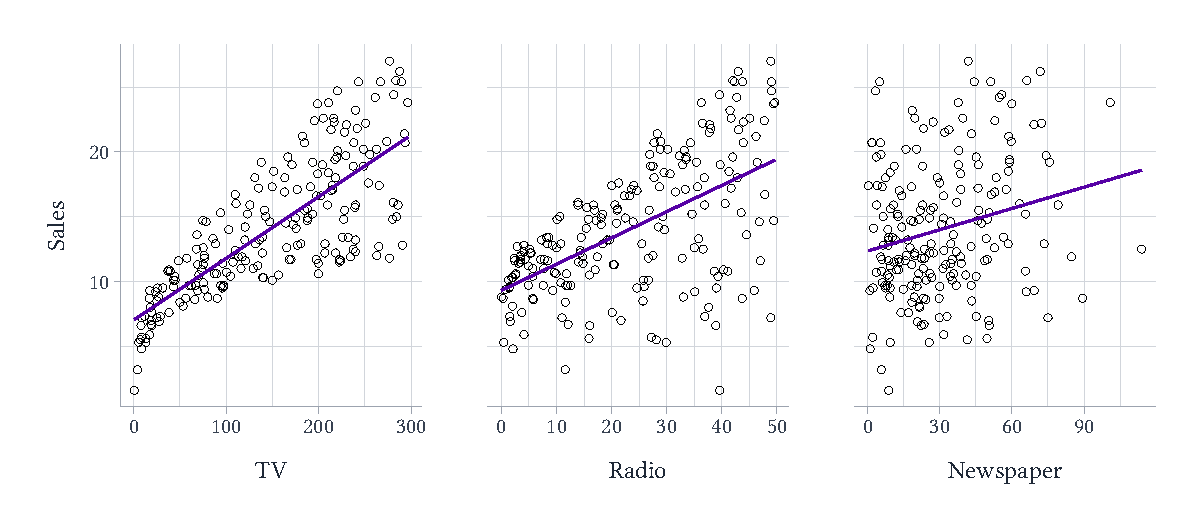
\includegraphics[width=\textwidth]{figures/sales_bivariate.pdf}
\end{frame}

\begin{frame}{}{}
  \bigskip
  \begin{center}
    \small
    \begin{tabular}{lcccc}
      \toprule
      Dependent Variable: & \multicolumn{4}{c}{Sales}\\
      \midrule
      Constant     & 7.033$^{***}$  & 9.312$^{***}$  & 12.35$^{***}$  & 2.939$^{***}$\\   
                    & (0.4578)       & (0.3882)       & (0.6338)       & (0.3365)\\   
      TV           & 0.0475$^{***}$ &                &                & 0.0458$^{***}$\\   
                    & (0.0027)       &                &                & (0.0019)\\   
      Radio        &                & 0.2025$^{***}$ &                & 0.1885$^{***}$\\   
                    &                & (0.0217)       &                & (0.0108)\\   
      Newspaper    &                &                & 0.0547$^{***}$ & -0.0010\\   
                    &                &                & (0.0186)       & (0.0064)\\   
      \midrule
      R$^2$        & 0.61188        & 0.33203        & 0.05212        & 0.89721\\  
      \bottomrule
    \end{tabular}
    \note[]{0.7\textwidth}{Signif. Codes: ***: 0.01, **: 0.05, *: 0.1}
  \end{center}
\end{frame}

\begin{frame}{Interpreting regression results}
  Notice on the last table, in the bivariate regression, higher newspaper ads spending is associated with higher sales


  \bigskip
  \emph{But}, after controlling for TV and Radio ads, there is no relationship between Newspaper ads and sales
  \begin{itemize}
    \item It seems like the bivariate relationship is being driven by newspaper ads being correlated with TV and Radio sales. 
    \begin{itemize}
      \item Holding them fixed removed the relationship between Newspaper ads and sales
    \end{itemize}
  \end{itemize}
\end{frame}

\begin{frame}{``All Else Equal''}
  The latin word you'll sometimes see is \emph{ceteris parabus} meaning ``other things being equal''.
  This refers to variables \emph{included} in your model
  \begin{itemize}
    \item In this case, we are ``holding fixed'' TV and Radio advertising
    
    \item Other things not included in the model still are moving as you compare areas with different Newspaper spending 
  \end{itemize}

  \bigskip
  For example, maybe cities with more newspaper spending have an older population than those with less
  \begin{itemize}
    \item OLS is assigning `credit' to Newspaper for the effect of different age distributions in a city on sales
  \end{itemize}
\end{frame}


\section{Regressors}

\subsection{Polynomials}

\begin{frame}{Quadratic terms}
  Say you have the following model with wages as a quadratic function of age
  $$
    w_i = \beta_0 + \beta_1 \text{age}_i + \beta_2 \text{age}_i^2 + u_i
  $$

  \bigskip
  Before we were discussing the idea of changing one variable, while holding the rest "equal"
  \begin{itemize}
    \item How does one change age without changing age$^2$?
  \end{itemize}

  \bigskip
  This was why I focused on separating the variables you condition on $X_i$ and the variables you include in your explanatory variables $W_i = \left( g_1(X_i), \dots, g_K(X_i) \right)'$
\end{frame}

\begin{frame}{Marginal Effects}
  $$
    \frac{\partial}{\partial x_\ell} \hat{f}(X) = \sum_{k=1}^K \frac{\partial}{\partial x_\ell} g_{k}(X) \hat{\beta}_{\text{OLS}, k}
  $$
  
  \bigskip
  This is holding fixed all the other variables at the original covariate values: $x_{1,i}, \dots, x_{K,i}$ and only changing $x_{\ell}$
  \begin{itemize}
    \item If a given $g_k$ does not depend on $x_\ell$, then $\frac{\partial}{\partial x_\ell} g_{k}(X) = 0$
    
    \item multiple $W_k$ can change from changing a particular $x_{\ell}$ 
  \end{itemize}
\end{frame}

\begin{frame}{Marginal effects with quadratic terms}
  \vspace{-\bigskipamount}
  $$
    \hat{w}_i = \hat{\beta}_0 + \hat{\beta}_1 \text{age}_i + \hat{\beta}_2 \text{age}_i^2
  $$

  \bigskip
  From calculus, we know that the partial derivative of $\hat{w}_i$ with respect to $\text{age}_i$ is given by 
  $$
    \frac{\partial}{\partial \text{age}_i} \hat{w}_i = \hat{\beta}_1 + 2 \hat{\beta_2} \text{age}_i
  $$
  
  \pause
  \bigskip
  The change in predicted wage of a worker as they age is given by $\hat{\beta}_1 + 2 \hat{\beta_2} \text{age}_i$ which depends on their age
  \begin{itemize}
    \item In words, how much predicted wages change as a worker gets a year older changes over a worker's lifetime
  \end{itemize}
\end{frame}

\imageframe{figures/ex_quadratic_cef.pdf}
\imageframe{figures/ex_linear_cef.pdf}
\imageframe{figures/ex_plogis_cef.pdf}

\begin{frame}{Testing quadratic term}
  \vspace{-\bigskipamount}
  $$
    \hat{w}_i = \hat{\beta}_0 + \hat{\beta}_1 \text{age}_i + \hat{\beta}_2 \text{age}_i^2
  $$

  \bigskip
  In general, a linear term is much easier to interpret than a quadratic term: `a one unit change is associated with a $\hat{\beta}_1$ unit change in $w$'
  \begin{itemize}
    \item We want to test whether the quadratic term is necessary or not
  \end{itemize}
\end{frame}

\begin{frame}{Testing quadratic term}
  \vspace{-\bigskipamount}
  $$
    \hat{w}_i = \hat{\beta}_0 + \hat{\beta}_1 \text{age}_i + \hat{\beta}_2 \text{age}_i^2
  $$

  \bigskip
  You can test whether there is a significant quadratic relationship by testing the null that $H_0: \beta_2 = 0$. Since we know $\hat{\beta}_2$ has a normal distribution, can use a $t$-test:
  $$
    \hat{t} \equiv \frac{\hat{\beta}_2 - 0}{\text{SE}(\hat{\beta}_2)}
  $$

  \bigskip
  If the $p$-value associated with this is larger than the level of significance, then we can not reject the simple linear model.
\end{frame}

\begin{frame}{Higher-order polynomials}
  This logic can be extended to higher-order polynomials to better estimate ``wiggly'' relationships between a given $X$ and $y$
  \begin{itemize}
    \item A key property of polynomials is that they are \alert{smooth} functions
    
    \item Any smooth CEF can be approximated well by a polynomial of high-enough order (Taylor expansion) 
  \end{itemize}

  \pause
  \bigskip
  The smoothness can be a feature if you think outcomes evolve smoothly with a given $X$
  \begin{itemize}
    \item But, it can be a problem if you think there's a discontinuity present (e.g. turing 21 has a large jump in rates of DUI)
  \end{itemize}
\end{frame}

\imageframe{figures/ex_jump_vs_polynomial.pdf}
\imageframe{figures/ex_jump_vs_polynomial_overfitting.pdf}

\begin{frame}{Polynomials and forecasting}
  One thing to note about polynomials is that they will always shoot off to $\pm \infty$ as you move $X \to$ $\infty$ and $-\infty$

  \bigskip
  When you forecast using your model \emph{outside} of the values of $X$ you train on, this is called \alert{extrapolation}
  \begin{itemize}
    \item Even for relatively small values outside the samples' \alert{domain} of $X$ can have very strange forecastes
  \end{itemize}

  \pause
  \bigskip
  The higher the order of the polynomial, the worse this gets
\end{frame}

\imageframe{figures/ex_extend_polynomial.pdf}
\imageframe{figures/ex_extend_polynomial_15.pdf}



\subsection{Indicators}

\begin{frame}{Intercept-only regression estimates sample mean}
  \begin{center}
    \texttt{feols(y \textasciitilde{} 1, data = df)}
  \end{center}

  \bigskip
  Running this regression is useful because it will estimate the mean of \texttt{y} and give us the standard error estimate $\frac{\hat{\sigma}}{\sqrt{n}}$
  \begin{itemize}
    \item This makes inference easier: hypothesis testing and confidence intervals 
  \end{itemize}
\end{frame}

\begin{frame}{Comparing means using indicator variables}
  An \emph{indicator variable} is a variable that can only equal $0$ and $1$, splitting units into groups
  \begin{itemize}
    \item $X$ "indicates" when a unit is of type 0 or type 1
    
    \item Often, it is written as $\one{\cdot}$ where `$\cdot$' is a true/false condition
  \end{itemize}

  \bigskip
  E.g. include
  \begin{itemize}
    \item being born male ($= 1$) or female ($= 0$)
    \item being White ($= 1$) or not ($= 0$)
    \item having a high-school degree ($= 1$) or not ($= 0$)
    \item $\one{\text{Height}_i \geq 6}$, being at least 6 foot tall
  \end{itemize} 
\end{frame}

\begin{frame}{Indicator variable}
  Let's work through some properties of an indicator variable, $D_i$. First, the sample mean of an indicator variable is the proportion of units with a 1:
  $$
    \frac{1}{n} \sum_{i=1}^n D_i = 
    \frac{\# \text{ of } 1{s}}{n} = 
    \text{\% of sample with } D_i = 1
  $$
  
  \pause
  \bigskip\bigskip
  Define $\pi$ as the (population) fraction of units with $D_i = 1$.
  Using the formula for variance, we can derive:
  $$
    \var(D_i) = \pi (1 - \pi)
  $$
\end{frame}

\begin{frame}{Covariance with an indicator variable}
  What is $\cov(D_i, Y_i)$? Rembmer
  $$
    \cov(D_i, Y_i) = \expec{D_i Y_i} - \expec{D_i} \expec{Y_i}
  $$
  
  \pause
  \bigskip
  Again, skipping the math:
  \begin{align*}
    \cov(D_i, Y_i) = \pi (1 - \pi) \left( \expec{Y_i}{D_i = 1} - \expec{Y_i}{D_i = 0} \right)
  \end{align*}
\end{frame}

\begin{frame}{Covariance with an indicator variable}
  Math details (if you're curious): 
  \begin{align*}
    \cov(D_i, Y_i) 
    &= \expec{D_i Y_i} - \expec{D_i} \expec{Y_i} \\
    &= \expec{D_i Y_i} - \pi \left( \pi \expec{Y_i}{D_i = 1} + (1 - \pi) \expec{Y_i}{D_i = 0} \right) \\
    &= \pi \expec{Y_i}{D_i = 1} - \pi \pi \expec{Y_i}{D_i = 1} - \pi (1 - \pi) \expec{Y_i}{D_i = 0} \\
    &= \pi (1 - \pi) \left( \expec{Y_i}{D_i = 1} - \expec{Y_i}{D_i = 0} \right)
  \end{align*}
\end{frame}

\begin{frame}{Regression with an indicator variable}
  Say you have a regression of $Y_i = \beta_0 + \beta_1 * D_i + u_i$. What does $\hat{\beta}_0$ and $\hat{\beta}_1$ equal?

  \begin{align*}
    \hat{\beta}_1 
    &= \frac{\cov(D_i, Y_i)}{\var{D_i}} \pause
    = \frac{\pi (1 - \pi) \left( \expec{Y_i}{D_i = 1} - \expec{Y_i}{D_i = 0} \right)}{\pi (1 - \pi)} \\
    &= \expec{Y_i}{D_i = 1} - \expec{Y_i}{D_i = 0}
  \end{align*}
  
  \bigskip
  The coefficient $\hat{\beta}_1$ tells me the difference in sample means between the group with $D_i = 1$ and the group with $D_i = 0$
\end{frame}

\begin{frame}{Regression with an indicator variable}
  Say you have a regression of $Y_i = \beta_0 + \beta_1 * D_i + u_i$. From the last slide, we have:
  $$ 
    \hat{\beta}_1 = \expec{Y_i}{D_i = 1} - \expec{Y_i}{D_i = 0} 
  $$

  \bigskip
  Solving our other first-order condition for $\hat{\beta}_0$, we have:
  \begin{align*}
    \beta_0 &= \expec{Y_i} - \hat{\beta}_1 \expec{D_i} \\
    &= \expec{Y_i} - \hat{\beta}_1 \pi \\
    &= \underbrace{\pi \expec{Y_i}{D_i = 1} + (1 - \pi) \expec{Y_i}{D_i = 0}} - \pi \expec{Y_i}{D_i = 1} - \pi \expec{Y_i}{D_i = 0} \\
    &= \expec{Y_i}{D_i = 0}
  \end{align*}
\end{frame}

\begin{frame}{Marginal effects}
  Our forecast is $\hat{Y}_i = \hat{\beta}_0 + \hat{\beta}_1 D_i$. Since $D_i$ can only be $0$ or $1$, our marginal effect just compares these values directly:
  \begin{align*}
    D_i = 0: &\quad\quad \hat{Y}_i = \hat{\beta}_0 + \hat{\beta}_1 * 0 = \hat{\beta}_0 \\
    D_i = 1: &\quad\quad \hat{Y}_i = \hat{\beta}_0 + \hat{\beta}_1 * 1 = \hat{\beta}_0 + \hat{\beta}_1 \\
  \end{align*}

  $\hat{\beta}_0$ is our predicted value for $Y_i$ for the group with $D_i = 0$ and $\hat{\beta}_0 + \hat{\beta}_1$ is our predicted value for $Y_i$ for the group with $D_i = 1$ 
  \begin{itemize}
    \item This makes $\hat{\beta}_1$ is the \emph{difference in the means} between those with $D_i = 1$ compared to $D_i = 0$
  \end{itemize}
\end{frame}

\begin{frame}{Interpreting coefficient on an indicator}
  Our forecast is $\hat{Y}_i = \hat{\beta}_0 + \hat{\beta}_1 D_i$. We can interpret $\hat{\beta}_1$ as follows:

  \begin{tcolorbox}[boxrule = 0pt, frame hidden, sharp corners, enhanced, borderline west = {2pt}{0pt}{zinc600}, interior hidden]
    ``On average, someone with $D_i = 1$ has a $\hat{\beta}_1$ larger/smaller value of $\hat{Y}$ compared to the units with $D_i = 0$ \emph{\color{blue} holding all else equal}''
  \end{tcolorbox}

  \begin{itemize}
    \item Where you add the last part if you include additional covariates
  \end{itemize}
\end{frame}

\begin{frame}{Example}
  Let's revisit our example with the \texttt{mtcars} dataset. There is an indicator variable, \texttt{am} for being an automatic ($= 1$) or manual ($= 0$). 
  Regress the miles per gallon a car gets, \texttt{mpg}, on \texttt{am}.

  \begin{itemize}
    \item In \texttt{fixest}, we can use \texttt{i(am)} to make it print out more nicely
  \end{itemize}
\end{frame}
 
\begin{frame}[fragile]{}
  \bigskip
  \begin{codeblock}
with(mtcars, mean(mpg[am == 0]))
#> [1] 17.14737
with(mtcars, mean(mpg[am == 1]) - mean(mpg[am == 0]))
#> [1] 7.24494

feols(mpg ~ i(am), data = mtcars)
#> OLS estimation, Dep. Var.: mpg
#> Observations: 32
#> Standard-errors: IID 
#>             Estimate Std. Error  t value   Pr(>|t|)    
#> (Intercept) 17.14737    1.12460 15.24749 1.1340e-15 ***
#> am::1        7.24494    1.76442  4.10613 2.8502e-04 ***
  \end{codeblock}
\end{frame}

\subsection{Multi-valued discrete variables}

\begin{frame}{Multi-valued discrete variables}
  This intuition will extend directly to settings where we have a discrete variable that obtains $K$ distinct values:
  \begin{itemize}
    \item E.g. race/ethnicity, 10-year bins of age, number of cylinders in engine
  \end{itemize}

  \pause
  \bigskip
  We can construct a \emph{set of} indicator variables for each value that $X$ can obtain. For $k = 1, \dots, K$
  $$
    X_{ik} \equiv \one{X_i = x_k}
  $$

  \bigskip
  There are $K$ such variables: $X_{i1}, \dots, X_{iK}$
\end{frame}

\begin{frame}{Multi-valued variable regression}
  \vspace*{-\bigskipamount}
  $$
    y_i = \sum_{k=1}^K X_{ik} \beta_k + u_i
  $$

  \bigskip
  From the same intuition as before, we have $\hat{\beta}_k$ is the sample average of $y_i$ for individuals with $X_i = x_k$
  \begin{itemize}
    \item We are in a very special case since these variables are mutually exclusive (only one of them is non-zero per unit), so this is easy to show with matrix algebra
  \end{itemize}
\end{frame}

\begin{frame}{Example}
  Let's revisit our example with the \texttt{mtcars} dataset. Let's see if \texttt{mpg} differs based on the number of cylinders a car has, \texttt{cyl}. 

  \begin{itemize}
    \item In \texttt{fixest}, we can use \texttt{i(cyl)} to make indicators for each value of a variable

    \item Otherwise, we could for $4$, $6$, and $8$ create the indicator variables with e.g. \texttt{mtcars\$cyl4 = (mtcars\$cyl == 4)}
  \end{itemize}
\end{frame}

\begin{frame}[fragile]{}
  Interpret these coefficients:

  \begin{codeblock}
feols(mpg ~ 0 + i(cyl), data = mtcars)
#> OLS estimation, Dep. Var.: mpg
#> Observations: 32
#> Standard-errors: IID 
#>        Estimate Std. Error t value   Pr(>|t|)    
#> cyl::4  26.6636   0.971801 27.4373  < 2.2e-16 ***
#> cyl::6  19.7429   1.218217 16.2064 4.4933e-16 ***
#> cyl::8  15.1000   0.861409 17.5294  < 2.2e-16 ***
#> ---
#> Signif. codes:  0 '***' 0.001 '**' 0.01 '*' 0.05 '.' 0.1 ' ' 1
#> RMSE: 3.0683   Adj. R2: 0.704784
  \end{codeblock}
\end{frame}

\begin{frame}{Intercept and Multicollinearity}
  In reality, we will want to include many predictor variables (beyond our single multi-valued discrete variable). 
  In this case, we want to include an \emph{intercept}

  \bigskip
  $$
    y_i = \beta_0 + \sum_{k=1}^K X_{ik} \beta_k + u_i
  $$
\end{frame}

\begin{frame}[fragile]{Multicollinearity}
  Our matrix $\bm{W}$ look like this. Note the 3 \texttt{cyl} indicator variables sum to the intercept
  \begin{codeblock}
#> (Intercept)   cyl::4   cyl::6   cyl::8
#>           1        0        1        0
#>           1        0        1        0
#>           1        1        0        0
#>           1        0        1        0
#>           1        0        0        1
#>           1        0        1        0
#>           1        0        0        1
#>           1        1        0        0
  \end{codeblock}
\end{frame}

\begin{frame}{Multicollinearity}
  \vspace*{-\bigskipamount}
  $$
    \hat{y}_i = \hat{\beta}_0 + \sum_{k=1}^K X_{ik} \hat{\beta}_k 
  $$

  \bigskip
  It turns out that we face a non-uniqueness problem because of the \alert{multicollinearity} we identified 
  \begin{itemize}
    \item We can add 10 to $\hat{\beta}_0$ and subtract 10 from $\hat{\beta}_4$, $\hat{\beta}_6$, and $\hat{\beta}_8$ and get the exact same $\hat{y}$
  \end{itemize}

  \bigskip
  Therefore, we will typically need to drop one of the $X_{ik}$ variables (or \texttt{R} will do it for you)
\end{frame}

\begin{frame}[fragile]{}
  \begin{codeblock}
feols(mpg ~ 1 + i(cyl), data = mtcars)
#> OLS estimation, Dep. Var.: mpg
#> Observations: 32
#> Standard-errors: IID 
#>              Estimate Std. Error  t value   Pr(>|t|)    
#> (Intercept)  26.66364   0.971801 27.43735  < 2.2e-16 ***
#> cyl::6       -6.92078   1.558348 -4.44110 1.1947e-04 ***
#> cyl::8      -11.56364   1.298623 -8.90453 8.5682e-10 ***
#> ---
#> Signif. codes:  0 '***' 0.001 '**' 0.01 '*' 0.05 '.' 0.1 ' ' 1
#> RMSE: 3.0683   Adj. R2: 0.714009
  \end{codeblock}
\end{frame}

\begin{frame}{Interpreting Multicollinearity}
  In the previous example, we dropped $\one{X_i = 4}$. This is the \alert{omitted group}. What happened to our coefficient estimates?

  \bigskip
  Just like in the indicator variable case, $\hat{\beta}_0$ estimated the mean of \texttt{mpg} for cars with $X_i = 4$
  
  \pause
  \bigskip
  The coefficients on the other $\hat{\beta}_k$ now represent the \emph{difference} in means between the group for $X_i = 6$ and the `omitted group' $X_i = 4$. 
  \begin{itemize}
    \item The mean for $X_i = 6$ is $19.742 = 26.663 - 6.921$
  \end{itemize}
\end{frame}

\begin{frame}[fragile]{Specifying \texttt{ref} option}
  \vspace*{-1.25\bigskipamount}
  \begin{codeblock}
feols(mpg ~ i(cyl, ref = 6), data = mtcars)
#> OLS estimation, Dep. Var.: mpg
#> Observations: 32
#> Standard-errors: IID 
#>             Estimate Std. Error  t value   Pr(>|t|)    
#> (Intercept) 19.74286    1.21822 16.20636 4.4933e-16 ***
#> cyl::4       6.92078    1.55835  4.44110 1.1947e-04 ***
#> cyl::8      -4.64286    1.49200 -3.11182 4.1522e-03 ** 
#> ---
#> Signif. codes:  0 '***' 0.001 '**' 0.01 '*' 0.05 '.' 0.1 ' ' 1
#> RMSE: 3.0683   Adj. R2: 0.714009
  \end{codeblock}
\end{frame}

\begin{frame}[fragile]{Significance with indicator variables}
  \vspace*{-1.25\bigskipamount}
  \begin{codeblock}
#>              Estimate Std. Error  t value   Pr(>|t|)    
#> (Intercept)  26.66364   0.971801 27.43735  < 2.2e-16 ***
#> cyl::6       -6.92078   1.558348 -4.44110 1.1947e-04 ***
#> cyl::8      -11.56364   1.298623 -8.90453 8.5682e-10 ***
#> ---
#> Signif. codes:  0 '***' 0.001 '**' 0.01 '*' 0.05 '.' 0.1 ' ' 1
  \end{codeblock}
  
  \bigskip
  Including an intercept also helps with certaint statistical inference.
  The estimates test that the average of $y$ for the omitted group is \emph{the same} for the other groups
  \begin{itemize}
    \item Rejecting this ($p$-value $< \alpha$) rejects the null that the two means are the same
  \end{itemize}
\end{frame}

\begin{frame}{Interpreting coefficient on indicators for a discrete variable}
  Our forecast is $\hat{Y}_i = \hat{\beta}_0 + \hat{\beta}_6 X_{i6} + \hat{\beta}_8 X_{i8}$. We can interpret $\hat{\beta}_6$ as follows:

  \begin{tcolorbox}[boxrule = 0pt, frame hidden, sharp corners, enhanced, borderline west = {2pt}{0pt}{zinc600}, interior hidden]
    ``On average, a car with $6$ cylinders has a $\hat{\beta}_6$ larger/smaller value of mpg compared to cars with $4$ cylinders \emph{\color{blue} holding all else equal}''
  \end{tcolorbox}

  \begin{itemize}
    \item Where you add the last part if you include additional covariates
  \end{itemize}
\end{frame}



\subsection{Interactions}

\begin{frame}{Why interactions}{Wages Example}
  Consider a model where we want to understand how wages are influenced by both being a female and being a college-educated worker. We can write the model as:
  $$
    w_i = \beta_0 + \beta_1 \text{female}_i + \beta_2 \text{college}_i + \beta_3 (\text{female}_i \times \text{college}_i) + u_i
  $$
  
  \bigskip
  Here, $\beta_3$ captures the interaction effect between female and college-education status on wages
  \begin{itemize}
    \item This means that the effect of females on wages may differ depending on whether the worker has a college-degree, and vice versa.
  \end{itemize}
\end{frame}

\begin{frame}{Interactions}{Wages Example}
  Consider the difference in predicted wages for non-college educated male vs. non-college educated workers:
  $$
    w_{i, NC,F} - w_{i, NC,M} = (\beta_0 + \beta_1) - \beta_0 = \beta_1
  $$

  \bigskip
  Compare this to the difference in predicted wages for college educated male vs. college educated workers:
  $$
    w_{i, C,F} - w_{i, C,M} = (\beta_0 + \beta_1 + \beta_2 + \beta_3) - (\beta_0 + \beta_2) = \beta_1 + \beta_3
  $$
\end{frame}

\begin{frame}{Interactions}{Wages Example}
  Wage-gap for college educated workers is $\beta_1 + \beta_3$ and the wage-gap for non-college educated workers is $\beta_1$
  \begin{itemize}
    \item $\beta_3$ represents the difference in wage gaps of college-educated vs. non-college-educated workers.
  \end{itemize}

  \pause
  \bigskip
  More generally, can interpret interactions how one variable changes the marginal effect of another variable
  \begin{itemize}
    \item This is similar to when you have a quadratic function of $X$, the marginal effect depends where you are along the distribution of $X$.
  \end{itemize}
\end{frame}


\begin{frame}{Interactions}{Partial Derivative}
  \vspace{-\bigskipamount}
  $$
    \hat{w}_i = \hat{\beta}_0 + \hat{\beta}_1 \text{female}_i + \hat{\beta}_2 \text{college}_i + \hat{\beta}_3 (\text{female}_i \times \text{college}_i) 
  $$
  
  \bigskip
  We can derive this result using partial derivatives:
  $$
    \frac{\partial \hat{w}_i}{\partial \text{female}_i} = 
    \hat{\beta}_1 + \hat{\beta}_3 \text{college}_i
  $$
  \pause
  In this case, it's a little weird to think of "small" changes in the female variable. Instead, we will think of it as a 1 unit change (from 0 to 1)
\end{frame}

\begin{frame}{Continuous interacted with a discrete variable}
  Let $X_i$ be a continuous variable and $D_i$ be a dummy variable and consider the regression
  $$
    y_i = \beta_0 + D_i \beta_1 + X_i \beta_2 + X_i D_i \beta_3 + u_i
  $$
  
  \pause
  \bigskip
  In this case, the marginal effect of $X_i$ is given by 
  $\frac{\partial \hat{y}_i}{\partial X_i} = \hat{\beta}_2 + D_i \hat{\beta}_3$ 
  \begin{itemize}
    \item The marginal effect for group $D_i = 0$ is given by $\hat{\beta}_2$
    \item The marginal effect for group $D_i = 1$ is given by $\hat{\beta}_2 + \hat{\beta}_3$
    
    \pause
    \item Therefore, $\hat{\beta}_3$ is the difference in marginal effects between $D_i = 1$ relative to $D_i = 0$
  \end{itemize}
\end{frame}


\begin{frame}{Continuous interacted with a discrete variable}
  \vspace*{-\bigskipamount}
  $$
    y_i = \beta_0 + D_i \beta_1 + X_i \beta_2 + X_i D_i \beta_3 + u_i
  $$
  
  \bigskip
  Exercise: 
  \begin{itemize}
    \item In words, how would you interpret a $t$-test for the null that $\hat{\beta}_2 = 0$?
    
    \item In words, how would you interpret a $t$-test for the null that $\hat{\beta}_3 = 0$?
  \end{itemize}
\end{frame}

\begin{frame}[fragile]{\texttt{mtcars} example}
  \vspace{-\bigskipamount}
  \begin{codeblock}[{}]
OLS estimation, Dep. Var.: mpg
              Estimate Std. Error   t value   Pr(>|t|)    
(Intercept) 26.624848   1.346754 19.769644  < 2.2e-16 ***
am::1        5.217653   2.324898  2.244250 3.2904e-02 *  
hp          -0.059137   0.008957 -6.602265 3.6781e-07 ***
am::1:hp     0.000403   0.013362  0.030152 9.7616e-01    
---
Signif. codes:  0 '***' 0.001 '**' 0.01 '*' 0.05 '.' 0.1 ' ' 1
  \end{codeblock}

  Exercise: Does the estimate relationship between being a car's horsepower and miles per gallon depend on whether it is an automatic? How do you know?
\end{frame}


\begin{frame}{Interaction terms always should have `main effects'}
  When including an interaction term, it is important to (almost) always include the \alert{main effects}

  \bigskip
  The \alert{main effects} are the variables by themselves. E.g. if you interact gender with race, you want to include race and gender as separate terms as well 
  \begin{itemize}
    \item The main effects are what let us interpret the interaction term as the `difference' in marginal effects
  \end{itemize}
\end{frame}

\begin{frame}{Continuous-Continuous interactions}
  Now consider two continuous variables being interacted:
  $$
    y_i = \beta_0 + X_{1,i} \beta_1 + X_{2,i} \beta_2 + X_{1,i} X_{2,i} \beta_3 + u_i
  $$
  
  \bigskip
  This is common when you think there are complementarities between variables 
  \begin{itemize}
    \item E.g. $y$ is crop-yield, $X_1$ is the amount of fertilizer applied, and $X_2$ is the amount of water given. Does it help to do more of both (complements)?
    
    \item $y$ is a measure of job performance, $X_1$ is a measure of on-the-job experience, and $X_2$ is a measure of training
  \end{itemize}
\end{frame}

\begin{frame}{Continuous-Continuous interactions}
  $$
    \frac{\partial \hat{y}_i}{\partial X_{1,i}} = \hat{\beta}_1 + X_{2,i} \hat{\beta}_3 
    \ \ \text{ and }\ \ 
    \frac{\partial \hat{y}_i}{\partial X_{2,i}} = \hat{\beta}_2 + X_{1,i} \hat{\beta}_3
  $$

  \bigskip
  Can interpret it in two ways:
  \begin{enumerate}
    \item The marginal effect of $X_{1}$ grows/shrinks with the value of $X_{2}$ (depending on the sign of $\hat{\beta}_3$)
  \end{enumerate}
\end{frame}

\subsection{Bins}

\begin{frame}{Key explanatory variables}
  In a forecast model, we might have a bunch of different variables we want to use as predictors

  \bigskip
  Many times, we really want to see how the forecasted outcome varies with a \emph{particular} variable of interest
  \begin{itemize}
    \item Want to ``control'' for a bunch of variables and then model the relationship between $y$ and key variable, $X_1$, flexibly
  \end{itemize}
\end{frame}

\begin{frame}{Partially-linear model}
  The \alert{Partially linear model} mixes high model flexibility in a key variable we care about and linear model for the rest of the covariates:
  $$
    y_i = \mu(X_{1i}) + W_i' \beta + u_i
  $$
  \vspace*{-\bigskipamount}
  \begin{itemize}
    \item $\mu(X_{1i})$ is a highly flexible function
    \item $W_i$ is a set of \emph{linear} control variables
  \end{itemize}

  \bigskip
  This allows you to prevent the curse of dimensionality by linearly controlling for most of the variables. 
  Allows a flexible model for the key variable of interest, $X_i$, that is good for graphing.
\end{frame}

\begin{frame}{Chopping $X_1$ into bins}
  The first approach, is to take $X_{1i}$ and make it into a discrete set of bins:
  \begin{itemize}
    \item E.g. Person's age into $20-24, 25-29, 30-34, \dots$
  \end{itemize}

  \bigskip
  Then, we can treat this as a multi-valued discrete variable
  \begin{itemize}
    \item Indicators for each bin and one omitted category
    
    \item We estimate sample means for each bin (relative to omitted group's mean)
  \end{itemize}
\end{frame}

\imageframe{figures/ex_bins_raw.pdf}
\imageframe{figures/ex_bins_split.pdf}
\imageframe{figures/ex_bins_estimate.pdf}
\imageframe{figures/ex_bins_compare_to_linear.pdf}
\imageframe{figures/ex_bins_add_polynomial.pdf}

\begin{frame}{Pros and Cons}
  One advantage is this is relatively easy to explain and quite flexible:
  \begin{itemize}
    \item ``The average property value for homes built from 1950 -- 1959 is $\$471,000$''
    
    \item If we want more flexibility, we can increase the number of bins (if we have enough data)
  \end{itemize}

  \pause
  \bigskip
  One problem with this method is that the marginal effect estimates can be odd:
  \begin{itemize}
    \item The estimated function is flat (0 marginal effect) except at the ``\alert{knots}'' where there is instant jump
    
    \item But, we are okay if we recognize this limitation
  \end{itemize}
\end{frame}




\subsection{Splines}

\begin{frame}{Previous approaches}
  \vspace*{-\bigskipamount}
  $$
    y_i = \mu(X_{1i}) + W_i' \beta + u_i
  $$

  We have discussed two ways to estimate $\mu(X_{1i})$ flexibly, both had pros and cons
  \begin{itemize}
    \item Polynomials allow for flexibility, but could become quite sensitive / noisy
    % TODO: add `noisy' in polynomial section
    
    \item Bins are flexible and simple to explain, but created artificial discontinuities and non-smoothness in our estimate
  \end{itemize}
\end{frame}

\begin{frame}{Previous approaches}
  \vspace*{-\bigskipamount}
  $$
    y_i = \mu(X_{1i}) + W_i' \beta + u_i
  $$

  \bigskip
  \alert{Splines} are a way to try and blend the two approaches:
  \begin{itemize}
    \item Chop up the domain of $X_1$ into a set of bins
    
    \item Within each bin, estimate a polynomial of a given order ($p$)
    
    \item Possibly, you can require the end points to ``connect'' ($s$)
  \end{itemize}
\end{frame}

\begin{frame}{Polynomial order and smoothness}
  Our binned averages is a particular version of splines:
  \begin{itemize}
    \item Polynomial of order 0 ($p = 0$)
    \item Not requied to connect ($s = 0$)
  \end{itemize}

  \bigskip
  We could increase the polynomial order to $p = 1$ to create linear functions within each bin
\end{frame}

\imageframe{figures/ex_bspline_p_1_s_0.pdf}

\begin{frame}{Polynomial order and smoothness}
  Our binned averages is a particular version of splines:
  \begin{itemize}
    \item Polynomial of order 0 ($p = 0$)
    \item Not requied to connect ($s = 0$)
  \end{itemize}

  \bigskip
  We could increase the polynomial order to $p = 1$ to create linear functions within each bin

  \bigskip
  If we want the lines to connect, we can add a smoothness constraint $s = 1$
\end{frame}

\imageframe{figures/ex_bspline_p_1_s_1.pdf}


\begin{frame}{Polynomial order and smoothness}
  Our binned averages is a particular version of splines:
  \begin{itemize}
    \item Polynomial of order 0 ($p = 0$)
    \item Not requied to connect ($s = 0$)
  \end{itemize}

  \bigskip
  We could increase the polynomial order to $p = 1$ to create linear functions within each bin

  \bigskip
  If we want the lines to connect, we can add a smoothness constraint $s = 1$

  \bigskip
  Or, we can set $p = 2$ and $s = 2$ to estimate quadratic functions and make them connect smoothly
\end{frame}

\imageframe{figures/ex_bspline_p_2_s_2.pdf}

\begin{frame}{Spline advantages and costs}
  From the previous figure, it seems like we've hit a really nice \emph{sweet spot}
  \begin{itemize}
    \item Quite flexible model to estimate $\mu(X_{1i})$ and can easily add covariates $W_i$ as controls
    
    \item But, we can not really do this with \emph{all} our covariates because splines add a lot of parameters (at least as many as bins you have)
  \end{itemize}

  \pause
  \bigskip
  It's not clear yet how we should chose the bins...
\end{frame}

% \begin{frame}{Splines Are ``Local''}
% 
% \end{frame}

\imageframe{figures/ex_bspline_few_knots.pdf}

\begin{frame}{Choosing Bins}
  There is a \emph{bias}/\emph{variance} trade-off when selecting the number of bins
  \begin{itemize}
    \item More bins means we can better approximate $\mu(X_{1i})$ (decreased bias)
    
    \item But, with fewer observations per bin, our estimates will be more noisy (increased variance)
  \end{itemize}

  \bigskip
  More, it is not clear why the bins should be evenly-space
  \begin{itemize}
    \item It makes `intuitive' sense, but maybe the bins should get smaller when the data is more `wiggly' and larger where the data is less
  \end{itemize}
\end{frame}


\begin{frame}{Choosing Bins}
  $$
    y_i = \mu(X_i) + W_i' \beta + u_i
  $$
  
  \bigskip
  One recent way of estimating this is using a `binscatter' regression:
  \begin{enumerate}
    \item Chop $X$ variable into $J$ bins with an \emph{equal number of observations into each bin}
    
    \item Choose $J$ \emph{optimally} to minimize mean-squared prediction error (bias-variance trade-off)
  \end{enumerate}

  \bigskip
  Implemented in the \texttt{binsreg} package
\end{frame}

\imageframe{figures/ex_bspline_binscatter.pdf}




\section{\texorpdfstring{$\log$}{log} transformations}

\begin{frame}{When to use $\log$ transformations}
  You should take the $\log$ of an outcome varible when you think a 1 unit change in $X$ is related to a \% change in $Y$. 
  
  \pause
  \bigskip
  Settings with skewed distributions (e.g. home prices, GDP, population, income)
  \begin{itemize}
    \item Skewness makes a `unit' change in $X$ difficult to think about
  \end{itemize}

  \pause
  \bigskip
  $\log(Y) = X\beta$ $\iff Y = e^{X\beta}$ is fitting an `exponential' relationship. These are common in:
  \begin{enumerate}
    \item Financial markets where compounding returns imply $Y_t = Y_0 e^{rt}$
    
    \item Epidemiology where disease growth rate is exponential (it is not actually, but early growth rate is approximately)
  \end{enumerate}
\end{frame}

\imageframe{figures/ex_log_y_raw.pdf}
\imageframe{figures/ex_log_y_log_vs_linear.pdf}

\begin{frame}{Extrapolating Exponential Relationship}
  If you thought extrapolating with polynomials with bad... Exponential is even more extreme
  \begin{itemize}
    \item Things that have rapid growth often will tend to slow-down
    
    \item Stonks don't go to the moon...
  \end{itemize}
\end{frame}


\begin{frame}{$\log$-transformation}
  \vspace*{-\bigskipamount}
  $$
    \log(\text{wages}_i) = \beta_0 + \beta_1 \text{College Degree}_i + u_i
  $$

  \bigskip
  This specification changes our interpretation of the slope coefficients:

  \begin{tcolorbox}[boxrule = 0pt, frame hidden, sharp corners, enhanced, borderline west = {2pt}{0pt}{zinc600}, interior hidden]
    ``Having a college degree is associated with an increase in wages of $\beta_1 * 100$ percent''
  \end{tcolorbox}
  
  \begin{itemize}
    \item E.g. if $\beta_1 = 0.02$, then a college degree is associated with a 2\% increase in wages.
  \end{itemize}

\end{frame}

\begin{frame}{Derivation of $\log$-transformation interpretation}
  Compare two individuals: unit $1$ with and unit $0$ without a college degree. Then, we have 
  \begin{align*}
    \log(\text{wages}_1) - \log(\text{wages}_0) &= 
    \beta_0 + \beta_1 - \beta_0 \\[1em]
    \implies \log(\text{wages}_1 / \text{wages}_0) &= \beta_1 \\[1em]
    \implies \log(1 + \frac{\text{wages}_1 - \text{wages}_0}{\text{wages}_0}) &= \beta_1
  \end{align*}

  \pause
  \bigskip
  If you recall, exponentiating gets rid of the the $\log$
  $$
    \frac{\text{wages}_1 - \text{wages}_0}{\text{wages}_0} = \exp(\beta_1) - 1
  $$
\end{frame}

\begin{frame}{Derivation of $\log$-transformation interpretation}
  The left-hand side is our percent-change formula from high-school science class
  $$
    \frac{\text{wages}_1 - \text{wages}_0}{\text{wages}_0} = \exp(\beta_1) - 1
  $$

  \pause
  \bigskip
  In this case, the more \emph{precise} answer is that having a college degree is associated with an $(\exp(\beta_1) - 1) * 100 \%$ change in $\text{wages}$
  \begin{itemize}
    \item But for $-0.10 < \beta_1 < 0.10$, $\exp(\beta_1) - 1$ is approximately equal to $\beta_1$ so it's simpler to use the latter
  \end{itemize}
\end{frame}

\imageframe{figures/pct_change_approximation.pdf}


% \begin{frame}{Example in \texttt{R}}
%   \begin{codeblock}
% library(fixest)
% feols(log(hp) ~ i(cyl), data = mtcars)
% #> OLS estimation, Dep. Var.: log(hp)
% #> Observations: 32
% #> Standard-errors: IID 
% #>             Estimate Std. Error  t value   Pr(>|t|)    
% #> (Intercept) 4.383896   0.069759 62.84353  < 2.2e-16 ***
% #> cyl::6      0.408183   0.111863  3.64895 1.0282e-03 ** 
% #> cyl::8      0.934249   0.093219 10.02206 6.2778e-11 ***
% #> ---
% #> Signif. codes:  0 '***' 0.001 '**' 0.01 '*' 0.05 '.' 0.1 ' ' 1
% #> RMSE: 0.220252   Adj. R2: 0.762984
%   \end{codeblock}
% \end{frame}



\begin{frame}{$\log$-$\log$ transformations}
  Alternatively, you may see $\log$ transformations of both variables:
  $$
    \log(Y_i) = \beta_0 + \beta_1 \log(X_i) + u_i
  $$

  \bigskip
  The interpretation is now simpler: a 1\% change in $X$ is associated with a $\beta_1$ \% change in $Y$
\end{frame}


\begin{frame}{Derivation}
  \vspace*{-1.5\bigskipamount}
  \begin{align*}
    \log(Y_1) - \log(Y_0) &= 
    \left( \beta_0 + \beta_1 \log(X_1) \right) - \left( \beta_0 + \beta_1 \log(X_0) \right) \\[1.5em]
    \implies \log(1 + \frac{Y_1 - Y_0}{Y_0}) &= 
    \beta_1 \log(1 + \frac{X_1 - X_0}{X_0}) \\[1.5em]
    \implies 1 + \frac{Y_1 - Y_0}{Y_0} &= 
    \left( 1 + \frac{X_1 - X_0}{X_0} \right)^{\beta_1} 
    \approx 1 + \beta_1 \frac{X_1 - X_0}{X_0} \\[1.5em]
    \implies \frac{Y_1 - Y_0}{Y_0} &= \beta_1 \frac{X_1 - X_0}{X_0}
  \end{align*}

\end{frame}

\imageframe{figures/log_log_approximation.pdf}

\begin{frame}{Near-perfect approximation}
  Our approximation is basically exact:
  $$
    \frac{Y_1 - Y_0}{Y_0} = \beta_1 \frac{X_1 - X_0}{X_0}
  $$

  \bigskip
  So, we interpret a $T$ percent increase in $X$ as a $\beta_1 * T$ percent increase in $Y$
\end{frame}
 

\begin{frame}{linear-$\log$ transformations}
  Last, we have the linear-$\log$ specification:
  $$
    Y_i = \beta_0 + \beta_1 \log(X_i) + u_i
  $$

  \bigskip
  This has the interpretation a 1\% change in $X$ is associated with a $\beta_1$ unit change in $Y$
\end{frame}



\section{Binary outcomes}

\begin{frame}{Binary Outcomes}
  In many instances, our outcome of interest is a \alert{binary outcome} taking the value of 0 or 1
  \begin{itemize}
    \item An indicator variable, but people call it a binary variable when it's an outcome
  \end{itemize}
  
  \bigskip
  E.g. $Y_i$ denoting whether a customer purchased something from a store and $X_i$ is demographic variables
  \begin{itemize}
    \item Want to predict the `propensity'/`probability' that someone will buy a product 
  \end{itemize}
\end{frame}

\begin{frame}{Expectation of a Binary Outcome}
  The expectation of a binary variable is just 
  \begin{align*}
    \expec{Y_i} &= 
    1 * \prob{Y_i = 1} + 0 * \prob{Y_i = 0} \\
    &= \prob{Y_i = 1}
  \end{align*}
  
  \bigskip
  This can be estimated by the sample proportion of times $Y_i = 1$:
  $$
    \hat{p} = \frac{1}{n} \sum_i Y_i
  $$
\end{frame}

\begin{frame}{Conditional Expectation Function of a Binary Outcome}
  The conditional expectation of a binary outcome can be found similarly:
  \begin{align*}
    \expec{Y_i}{X_i = x} &= 
    1 * \prob{Y_i = 1}{X_i = x} + 0 * \prob{Y_i = 0}{X_i = x} \\
    &= \prob{Y_i = 1}{X_i = x}
  \end{align*}
  
  \bigskip
  We can estimate the CEF of a binary outcome at a point $x$ in the same way:
  \begin{itemize}
    \item Subset to people with $X_i = x$
    \item Take the sample proportion of $Y_i = 1$ \emph{within that subsample}. Call this $\hat{f}(x)$
  \end{itemize}
\end{frame}

\begin{frame}{Conditional Expectation Function of a Binary Outcome}
  Note that this procedure faces the same benefits and costs as with a continuous outcome variable:
  \begin{itemize}
    \item The estimator is unbiased and consistent 
    
    \item But the curse of dimensionality makes this estimator noisy when $X_i$ has a large number of variables
  \end{itemize}
  
  \pause
  \bigskip
  This motivates us to study a linear model for the conditional expectation function:
  $$
    \expec{Y_i}{X_i = x} = \prob{Y_i = 1}{X_i = x} = W_i' \beta
  $$
  for some $W_i = g(X_i)$
\end{frame}

\begin{frame}{Linear Probability Model}
  This motivates us to study a linear model for the conditional expectation function:
  $$
    \expec{Y_i}{X_i = x} = \prob{Y_i = 1}{X_i = x} = W_i' \beta
  $$
  for some $W_i = g(X_i)$

  \bigskip\bigskip
  This is called a \alert{linear probability model} and predicts the proportion of $1$s you would observe in the population given $X_i = x$
  \begin{itemize}
    \item Can be estimated in the exact same way $\hat{\beta}_{\text{OLS}} = \left( \bm{W}' \bm{W} \right)^{-1} \bm{W}' \bm{Y}$
  \end{itemize}
\end{frame}

\begin{frame}{Marginal Effect Interpretation}
  Our marginal predictive effects take the same form:
  $$
    \frac{\partial}{\partial x_\ell} \probhat{Y_i = 1}{X_i = x} = \sum_{k=1}^K \frac{\partial}{\partial x_\ell} g_{k}(X) \hat{\beta}_{\text{OLS}, k}
  $$
  
  \bigskip
  You should reword the interpretation to reflect that you are estimating the conditional probability of $Y_i = 1$:

  \begin{tcolorbox}[boxrule = 0pt, frame hidden, sharp corners, enhanced, borderline west = {2pt}{0pt}{zinc600}, interior hidden]
    ``On average, a one unit increase in $x_\ell$ is associated with a $\hat{\beta}_1$ larger/smaller probability of $Y_i = 1$ \emph{\color{blue} holding all else equal}''
  \end{tcolorbox}
\end{frame}

\begin{frame}{Problems with Linear Probability Model}
  \vspace*{-\bigskipamount}
  $$
    \expec{Y_i}{X_i = x} = \prob{Y_i = 1}{X_i = x} = W_i' \beta
  $$

  \bigskip
  Probabilities must fall between 0 and 1. When we estimate our model, we do not impose that \emph{restriction}
  \begin{itemize}
    \item For given values of $x$, $w' \hat{\beta}_{\text{OLS}}$ can be less than 0 or greater than 1
  \end{itemize}

  \bigskip
  Though, it is worth saying that this is \emph{not} true when you \emph{only} use indicator variables in $W_i$
\end{frame}

\begin{frame}{Logistic Regression}
  Instead, we will use a \alert{logistic transformation} to model the conditional probability:
  \bigskip
  $$
    \expec{Y_i}{X_i = x} = \prob{Y_i = 1}{X_i = x} = 
    \tcbhighmath[colback = bgGreen]{\textrm{logistic}} 
    \left(\tcbhighmath[colback = bgPurple]{W_i' \beta}\right)
  $$

  % \devgrid
  \begin{tikzpicture}[remember picture, overlay]
    \node [anchor = north, text width = 0.25\textwidth] at (page cs:0.65,0.365) {
      \begin{center}
        \setstretch{0.8}
        {\footnotesize\color{green} ``transformation''}
      \end{center}
    };
    \node [anchor = south, text width = 0.25\textwidth] at (page cs:0.73,0.325) {
      \begin{center}
        \setstretch{0.8}
        {\footnotesize\color{purple} ``Linear Index''}
      \end{center}
    };
  \end{tikzpicture}

  \smallskip
  where $\logistic{W_i'\beta} = \frac{e^{W_i'\beta}}{e^{W_i'\beta} + 1}$ and $W_i' \beta$ is called the (linear) `index function'

  \pause
  \begin{itemize}
    \item The $\textrm{logistic}$ function ensures that the forecasted probabilities fall within 0 and 1
  \end{itemize}
\end{frame}

\imageframe{figures/logistic_link_function.pdf}

\begin{frame}{Binary Choice Model}
  One way to arrive at the logistic model is to assume a \alert{latent index model} where:
  $$
    Y_{i}^* = \tcbhighmath[colback = bgPurple]{W_i' \beta} + \varepsilon_i
  $$

  \bigskip
  When the `utility' $Y_i^*$ is high-enough, we switch from $0$ to $1$. 
  We observe $Y_i \equiv \one{Y_i^* \geq 0}$.
\end{frame}

\begin{frame}{Binary Choice Model $\implies$ Logistic CEF}
  \vspace*{-\bigskipamount}
  $$
    Y_{i}^* = \tcbhighmath[colback = bgPurple]{W_i' \beta} + \varepsilon_i 
    \quad \text{ and } \quad 
    Y_i \equiv \one{Y_i^* \geq 0}
  $$

  \bigskip
  When $\varepsilon_i$ follows the \alert{logistic distribution}, this implies 
  $$
    \prob{Y_i = 1}{X_i} = 
    \prob{\varepsilon_i \leq - \tcbhighmath[colback = bgPurple]{W_i' \beta}} = 
    \frac{e^{W_i'\beta}}{e^{W_i'\beta} + 1}
  $$

  \pause
  \bigskip
  \bigskip
  That is, our latent-index model and a logistic error term implies our logistic transformation
  \begin{itemize}
    \item If we assume $\varepsilon_i$ is normally distributed, then we end up with a ``probit''
  \end{itemize}
\end{frame}

\begin{frame}{``Likelihood''}
  \vspace*{-\bigskipamount}
  $$
    \prob{Y_i = 1}{X_i} = 
    \prob{\varepsilon_i \leq - \tcbhighmath[colback = bgPurple]{W_i' \beta}} = 
    \frac{e^{W_i'\beta}}{e^{W_i'\beta} + 1}
  $$

  \bigskip
  With this, we can think of each $Y_i$ as a Bernoulli random variable with probability of success of $\pi_i \equiv \frac{e^{W_i'\beta}}{e^{W_i'\beta} + 1}$

  \pause
  \bigskip
  \bigskip
  The \alert{likelihood} of observing $Y_i = 1$ is $\pi_i$ and the \alert{likelihood} of observing $Y_i = 0$ is $1 - \pi_i$
  \begin{itemize}
    \item The $\pi_i$ depends on our choice of $\beta$
  \end{itemize}
\end{frame}

\begin{frame}{Maximum-Likelihood Estimation}
  If our outcomes, $Y_i$, are independent, then our likelihood of observing the full vector $Y$ given $\beta$ is
  $$
    \mathcal{L}(\beta \ \vert \ Y, \bm{X}) = \prod_{i=1}^n 
    \ \tcbhighmath[colback = bgGreen]{\pi_i^{Y_i}} \
    \tcbhighmath[colback = bgPurple]{(1 - \pi_i)^{1 - Y_i}}
  $$

  Recall $\pi_i \equiv e^{W_i'\beta} / ( e^{W_i'\beta} + 1 )$

  % \devgrid
  \begin{tikzpicture}[remember picture, overlay]
    \node [anchor = north, text width = 0.25\textwidth] at (page cs:0.59,0.405) {
      \begin{center}
        \setstretch{0.8}
        {\footnotesize\color{green} $= 1$ when $Y_i = 0$}
      \end{center}
    };
    \node [anchor = south, text width = 0.25\textwidth] at (page cs:0.65,0.36) {
      \begin{center}
        \setstretch{0.8}
        {\footnotesize\color{purple} $= 1$ when $Y_i = 1$}
      \end{center}
    };
  \end{tikzpicture}

  \pause
  \bigskip
  The goal then is to find the best $\beta$ to \emph{maximize} the \emph{likelihood} of observing the data $Y$ we did observe
\end{frame}

\begin{frame}{Maximum-Likelihood Estimation In R}
  Luckily, our \texttt{fixest} package also makes performing logistic regression simple: 
  
  \texttt{feglm(fmla, data, family = "logit")}

  This performs maximum-likelihood estimation of $\hat{\beta}$
\end{frame}

\begin{frame}{Forecasting probabilities}
  With our estimated $\hat{\beta}$, we can form forecasts of 
  $$
    \hat{\pi}_i \equiv e^{W_i' \hat{\beta}} / ( e^{W_i' \hat{\beta}} + 1 )
  $$

  \bigskip
  Note here, we are predicting \emph{the probability} that $Y_i = 1$ given that $X_i = x$. 
  \begin{itemize}
    \item Often, this is interesting (60\% of people buy this product when $X_i = x$)
    \item If we were forced, could chose a rule like $\hat{Y}_i = 1$ if $\hat{\pi}_i \geq 0.5$
  \end{itemize}

  \pause
  \bigskip
  Forecasting can be done easily as well with our \texttt{predict} function and possibly with the \texttt{newdata} argument
\end{frame}

\begin{frame}{Marginal Effects Of Logistic Transformation}
  Remember that our ``index'' is given by our linear function $U_i = W_i' \beta$. 

  \bigskip
  We know how to calculate marginal effects of $U_i$ with respect to some $x_{i,\ell}$: 
  $$
    \frac{\partial}{\partial x_{\ell}} \hat{U}_i = \sum_k \frac{\partial}{\partial x_{\ell}} g_k(\ell) \hat{\beta}_\ell
  $$

  \pause
  \bigskip
  But, $\hat{\pi}_i = e^{\hat{U}_i} / ( e^{\hat{U}_i} + 1 )$ is a transformation of $\hat{U}_i$
  \begin{itemize}
    \item How does $\hat{\pi}_i$ change with $\hat{U}_i$?
  \end{itemize}
\end{frame}

\imageframe{figures/logistic_marginal_effect.pdf}

\begin{frame}{Marginal Effects Of Logistic Transformation}
  \vspace*{-\bigskipamount}
  $$
    \hat{\pi}_i = e^{\hat{U}_i} / ( e^{\hat{U}_i} + 1 )
  $$
  
  \bigskip
  % https://en.wikipedia.org/wiki/Logistic_function#Derivative
  The partial derivative can be estimated via the chain-rule:
  $$
    \frac{\partial}{\partial x_{\ell}} \hat{\pi}_i =
    \frac{e^{\hat{U}_i}}{(e^{\hat{U}_i} + 1)^2} * 
    \frac{\partial}{\partial x_{\ell}} \hat{U}_i
  $$
\end{frame}

\begin{frame}{\texttt{marginaleffects} Package In R}
  This would be a bit of a pain to estimate by hand
  \begin{itemize}
    \item And even more annoying would be getting standard errors!
  \end{itemize}

  \bigskip
  But, the \texttt{marginaleffects} package makes this really easy (and works with fixest!)
  \begin{itemize}
    \item See \url{https://marginaleffects.com/chapters/slopes.html} for details
  \end{itemize}
\end{frame}

\begin{frame}{Marginal Effects}
  Once we calculate the marginal effect, $\frac{\partial}{\partial x_{\ell}} \hat{\pi}_i$, we would interpret it as 

  \begin{tcolorbox}[boxrule = 0pt, frame hidden, sharp corners, enhanced, borderline west = {2pt}{0pt}{zinc600}, interior hidden]
    ``On average, for a unit with $X_i = x$, a one unit larger $x_{i, \ell}$ is associated with an increased probability of $Y_i = 1$ of \# \emph{\color{blue} holding all else equal}''
  \end{tcolorbox}

  \pause
  \bigskip
  Notice now the marginal effect depends on the full set of covariates $X_i = x$ (because they all impact $W_i' \beta$), we need to specify all of this when we talk about marginal effects
\end{frame}

\begin{frame}{Interpreting Marginal Effects}
  Notice now the marginal effect depends on the full set of covariates $X_i = x$ (because they all impact $W_i' \beta$), we need to specify all of this when we talk about marginal effects

  \bigskip
  Two options people use:
  \begin{itemize}
    \item Specify $x$ to be the sample mean of each $X_i$; 
    \begin{itemize}
      \item ``At the mean of $X$, the marginal effect is $\dots$''
    \end{itemize}

    \medskip
    \item Average the marginal effect across the sample or a particular sub-sample
    \begin{itemize}
      \item ``On average for men, the marginal effect of increasing $x_{i,\ell}$ is $\dots$''
    \end{itemize}
  \end{itemize}
\end{frame}


\begin{frame}[fragile]{R Example -- Estimation}
  \begin{codeblock}
library(fixest)
est <- feglm(am ~ mpg, data = mtcars, family = "logit")
print(est)
#> GLM estimation, family = binomial(link = "logit"), Dep. Var.: am
#> Observations: 32
#> Standard-errors: IID 
#>              Estimate Std. Error  z value  Pr(>|z|)    
#> (Intercept) -6.603527   2.390311 -2.76262 0.0057339 ** 
#> mpg          0.307028   0.116740  2.63002 0.0085380 ** 
#> ---
#> Signif. codes:  0 '***' 0.001 '**' 0.01 '*' 0.05 '.' 0.1 ' ' 1
  \end{codeblock}
\end{frame}

\imageframe{figures/mtcars_forecast.pdf}

\begin{frame}[fragile]{R Example -- Forecasting}
  \begin{codeblock}
head(predict(est))
#> [1] 0.46109512 0.46109512 0.59789839 0.49171990 0.29690087 

predict(est, newdata = data.frame(mpg = c(20, 25, 30)))
#> [1] 0.3862832 0.7450109 0.9313311
  \end{codeblock}
\end{frame}

\begin{frame}[fragile]{R Example -- Marginal Effects}
  \begin{codeblock}
library(marginaleffects)
slopes(
  est, variables = "mpg",
  newdata = data.frame(mpg = c(20, 25, 30))
)
#> Estimate  Std. Error     z  Pr(>|z|)     S     2.5 %  97.5 %
#>   0.0728      0.0285  2.55    0.0108   6.5   0.01684  0.1287
#>   0.0583      0.0144  4.05    <0.001  14.2   0.03007  0.0866
#>   0.0196      0.0144  1.36    0.1738   2.5  -0.00866  0.0479
  \end{codeblock}
\end{frame}

\imageframe{figures/mtcars_forecast.pdf}










\end{document}
